%%%% ijcai11.tex

\typeout{IJCAI-11 Instructions for Authors}


% These are the instructions for authors for IJCAI-11.
% They are the same as the ones for IJCAI-07 with superficical wording
%   changes only.

\documentclass{article}
% The file ijcai11.sty is the style file for IJCAI-11 (same as ijcai07.sty).

\usepackage{graphicx}
\usepackage{ijcai11}
\usepackage{float}
%\floatstyle{boxed}
\restylefloat{figure}

% Use the postscript times font!
\usepackage{times}

% the following package is optional:
%\usepackage{latexsym} 

% Following comment is from ijcai97-submit.tex:
% The preparation of these files was supported by Schlumberger Palo Alto
% Research, AT\&T Bell Laboratories, and Morgan Kaufmann Publishers.
% Shirley Jowell, of Morgan Kaufmann Publishers, and Peter F.
% Patel-Schneider, of AT\&T Bell Laboratories collaborated on their
% preparation.

% These instructions can be modified and used in other conferences as long
% as credit to the authors and supporting agencies is retained, this notice
% is not changed, and further modification or reuse is not restricted.
% Neither Shirley Jowell nor Peter F. Patel-Schneider can be listed as
% contacts for providing assistance without their prior permission.

% To use for other conferences, change references to files and the
% conference appropriate and use other authors, contacts, publishers, and
% organizations.
% Also change the deadline and address for returning papers and the length and
% page charge instructions.
% Put where the files are available in the appropriate places.


\title{Increasing Productivity in HPC by changing Scheduler Policy based on I/O Bandwidth
}
\author{Dineshkumar Rajagopal(dineshkumar.rajagopal@ensimag.grenoble-inp.fr) \\ 
 M1 MoSIG-ENSIMAG,MESCAL-INRIA Lab-Grenoble.\\
Supervised by:Olivier Richard(olivier.richard@imag.fr)} % Mosig student

\begin{document}
\maketitle
\begin{abstract}

Present days High Performance Computing(HPC) Architecture sharing Distributed File Systems ({\em eg.PVFS,NFS,CLUSTER})\cite{Distributed_File_System} with the hundreds of thousands of computing nodes at the same time. This sharing causes heavy I/O contention, when simultaneous requests from different applications. High I/O contention will degrade the performance and productivity machine wide. This paper focuses on changing the scheduling methodology based on I/O Bandwidth requirements of each application to reduce I/O contention, and increase the productivity and performance. We Performed experiment with IOR\cite{IOR_Description}\cite{IOR_Performance_measurement_in_File_System} Benchmark to compare the systems Productivity and File system Performance in the OAR\cite{inproceedingscapit.cd-cghmmnr_bswhlc_05} Batch Scheduler in GRID’5000\cite{Grid5000} Environment.  The Result shows the Productivity improvement in the new scheduling approach.

\end{abstract}
\section{Introduction}
\paragraph{}Increasing the power of HPC from PetaScale to ExaScale is not only by increasing the performance of computing to exaFLOPS(measuring performance of computing system). Performance of HPC affected by many factors some of them are I/O contention, HPC Architecture, Topology of Network, Network links between nodes, Number of nodes in HPC and current workload of the system. But in this paper we focus on Reducing I/O contention to improve Productivity of the HPC system.


Present days scientific computations has to perform more computation on data, so I/O operations requirement increased from KB/s to MB/s may be in the future it would be TB/s. Even though high I/O tasks are running in the HPC system, fifty percentage of submitted jobs in the GRID’5000 are low I/O\cite{lallouette:hal-00967106}, So we have to satisfy all the applications I/O requirements. Resolving the problem by naively increasing the  Distributed File System speed and requirements with the new technology is not a good solution. Because in the future Number of Processes(Number of Users) will be increased as well Speed of  Computing will be higher than I/O speed so I/O contention remain unfixed (Historical evolution of I/O speed is much slower than Processor computing speed).


In the beginning I/O optimization is the technique to reduce I/O contention. But it was failed  for so many reasons one of the reason is optimization performed in the different levels from Application side coding(using MPI-IO,HDF5 libraries) to Network request to File system Scheduler independently, so one optimization will affect another and lose the optimization globally. As well optimization techniques try fair I/O response to the simultaneous applications irrespective of the applications I/O requirements so I/O contention increase while two high I/O Jobs request data from the shared file system.


When the multiple processes running on the HPC(Heavy workload) may decay the performance and productivity Because of I/O contention. As well real performance of HPC is not running a single application in the speed of HPC. It has to support multiple processes, so reducing I/O contention is the challenging problem in HPC.


The bottleneck of I/O contention and multiple processes are inseparable. Segregating the Jobs(Processes) with the I/O requirements ,High and Low I/O Jobs and scheduling them by combining low I/O jobs with low or high I/O jobs to satisfy the overall I/O bandwidth of the Distributed File System to increase the productivity of the System machine wide.


The rest of this paper is organized as follows. \textbf{Section 1. I/O contention and the effects in the HPC system} covers How we organized the experiment with the Batch Scheduler OAR(RJMS in Grid’5000) with IOR benchmark(for testing Parallel File Systems Performance) to measure the I/O contention variation with different Jobs running Simultaneously and the effects of I/O contention machine wide. \textbf{ Section 2.Scheduling Policy based on I/O Bandwidth } covers How we changed the Batch Scheduler OAR to Support I/O Bandwidth and reduce I/O contention and compare performance with the Previous scheduling  Policy. In \textbf{Section 3} we concluded with the results we obtained and In \textbf{Section 4 }we proposed the Future work.
\section{I/O contention and the effects in the HPC system}
\paragraph{}Contention is always happened in the shared resource because of the competition for accessing the shared resource. In our HPC architecture distributed file system is shared with the large number of Computing nodes so I/O contention is not ignorable. I/O contention reduces the I/O Bandwidth (MB/s), so Computation is waiting for the I/O response. Present days scientific computations are highly depended on the I/O operations to complete Jobs,so reducing I/O contention will increase the performance of the jobs individually. I/O contention causes computation cycle idle(because of I/O response slow) so usage of the resources (processor) are not efficient and time taken to finish the job is delayed and varied with the I/O contention rate.


For testing the I/O contention and scheduler we used docker-oar cluster[7] and  created the virtual cluster like environment in the single computer and submitted Jobs with the  varying I/O operations(high and low) to analyze the I/O contention behavior based on the Jobs I/O operations. %requirements(I/O operations) of  theJobs.


Why we selected the Docker to deploy the cluster like environment in the Single Machine(Computer Node) is,{\em we can easily develop, build and deploy Distributed Applications easily}\cite{docker-oar}\cite{docker}. We deployed a cluster with four Computing Nodes, Frontend and Server(Handling the Real Batch Scheduling and giving the interface for the Job submission)\cite{inproceedingscapit.cd-cghmmnr_bswhlc_05} and NFS Server for Distributed File System. This cluster Architecture is shown in the figure 1.
\newline
\begin{figure}
  \centering    
      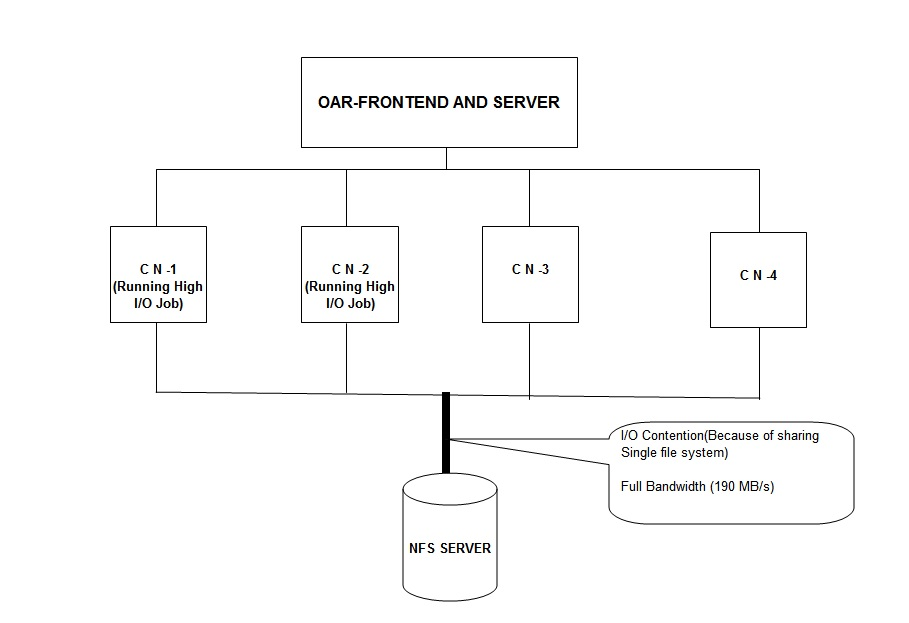
\includegraphics[width=0.5\textwidth]{CusterArchitecture-exp.jpg}
  \caption{This is the cluster was deployed in the single machine for doing all the experiments, In the figure you can see the I/O contention is happening in the Shared Network medium. }
\end{figure}
In the Frontend users can Submit the Jobs with their resource requirements(eg. oarsub -l nodes=1,walltime=1:00:00 (job-name))to finish the job. Server will check the requirements and the available resources to put the jobs in the Specific queue. More details of the OAR\cite{inproceedingscapit.cd-cghmmnr_bswhlc_05} Scheduler is outside the scope of this paper. Job submission command is only considering the {\typebf Computing nodes} as the resource irrespective of Jobs I/O requirement so I/O contention is not ignorable. For the I/O contention analyze we used two Jobs one is High I/O(it will write 500MB in a shared NFS sever file) and another one is Low I/O(it will write 50MB in a shared NFS sever file). We run the Jobs with the various combinations and measured I/O bandwidth usage for each Jobs and time to finish the Jobs for each applications.
\newline 
\begin{figure}
  \centering    
      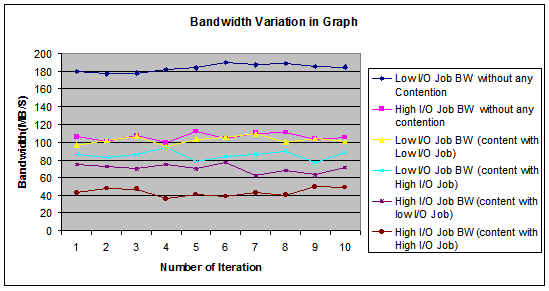
\includegraphics[width=0.5\textwidth]{BandwidthVariationinLine.png}
  \caption{Shows Various Jobs I/O Bandwidth variation due to I/O contention. In that two High I/O Jobs run simultaneously then only the I/O bandwidth is very low and I/O contention is high, So avoiding this combination will reduce I/O contention drastically.}
\end{figure}
Various combinations we choosed for the experiments are \typebf { 1) High I/O job run alone(without any I/O contention) 2) Low I/O job run alone(without any I/O contention) 3) High I/O job run with another High I/O job simultaneously(high I/O contention occurred) 4) High I/O job run with Low I/O job simultaneously(Medium I/O contention Occurred) 5) Low I/O job run with another Low I/O job simultaneously(Low I/O contention Occurred) }. The variation with the I/O rate(I/O Bandwidth) is shown in the Figure -2. From the Figure-2 and Figure-3 we can infer the idea that most of the I/O contention due to the High I/O Job run with another High I/O Job, So avoiding that combination of Job allocation will decrease the I/O contention drastically. 
\newline
\begin{figure}
  \centering    
      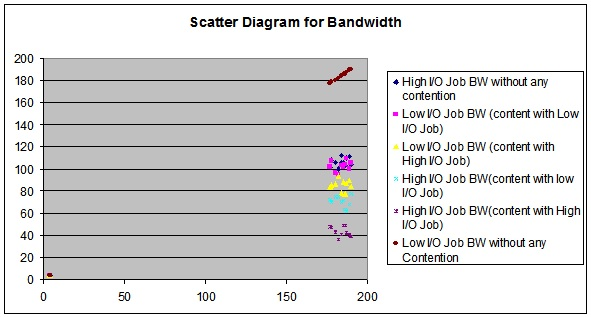
\includegraphics[width=0.5\textwidth]{ScatterDiagram.jpg}
  \caption{This is the scatter graph for the I/O Bandwidth for the different Job combinations. In this figure we can see High I/O jobs I/O bandwidth is very low while it content with another High I/O job.}
\end{figure}
\begin{figure}
  \centering    
      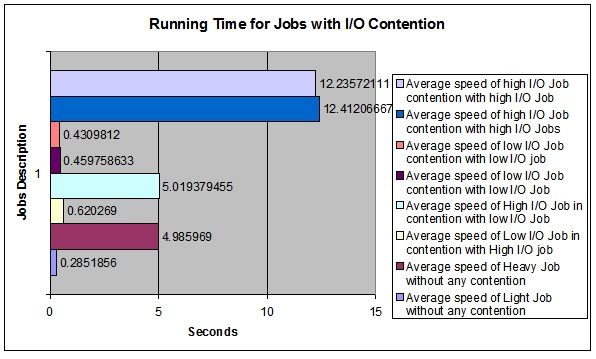
\includegraphics[width=0.5\textwidth]{RunningTime-I-O-Contention.jpg}
  \caption{Various Job combinations running time variation due to I/O contention. In that two High I/O Jobs running simultaneously take 2.5 times the High I/O Job running alone without any contention, so avoiding this situation will reduce I/O contention drastically.}
\end{figure} 


I/O contention decreased I/O bandwidth based on the combinations of I/O based Jobs running at the same time, so most of the situation Computing cycle is in idle for the wrong Combination of Multiple Jobs running Simultaneously. This will affect the productivity and performance of the Jobs. In Figure-4 we can get the information of the running time of each Jobs. Running Time is taking more computing cycles for High I/O tasks than all the Low I/O tasks as well when two simultaneous High I/O running time is 2.5 times the running time of High I/O job running alone(without any contention). Usually when one Job take 1 seconds to finish the work, then the two jobs running simultaneously in the two computing nodes it should be finished in 1 second because two jobs are in the two different machines. In the above simultaneous High I/O Jobs 1.5 times wastage of Computing Cycle in the Computing Nodes due to the low I/O response(because of High I/O contention) from the Shared File system. In the other Job Combinations Running Time is faster than the two High I/O jobs in simultaneous, so in the new Scheduling Policy we will avoid this combination to allocate the Jobs.
\newline 
\begin{figure}
  \centering    
      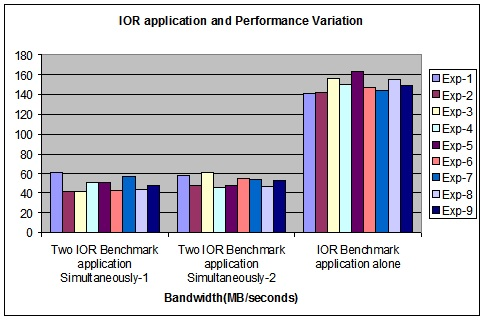
\includegraphics[width=0.5\textwidth]{IOR-Application-Performance.jpg}
  \caption{Two IOR applications simultaneously run in the System and Compared the I/O contention Result with the Previous result it shows I/O optimization at the Application Level does not resolve the I/O contention}
\end{figure}


In our test Jobs High and Low I/O are not optimized in the application side using MPI-IO Libraries, So we did Test with the IOR(Interleaved-or-Random) Benchmark application and compared the results with the previous results,but both are correlated. We wrote IOR script with the specification of doing test repetition 10, Buffer Size 25MB, File Size to Write 500MB, by passing cache, Single Shared File. With the IOR script specification we did test nine times. Same IOR test we did with another IOR application run in the another Computing Node simultaneously and plotted the Results in Figure-5 and Figure-6. From the IOR results High I/O operations will increase I/O contention Same as the previous test without application I/O optimization. From this result, We can get the information I/O optimization performed in the application side does not reduce I/O contention and it remains unresolved. Avoiding those High I/O contention situation by changing the scheduling policy based on I/O Bandwidth requirements. Considered I/O bandwidth as the resource as Computing nodes to allocate the Jobs.
\newline
\begin{figure}
  \centering    
      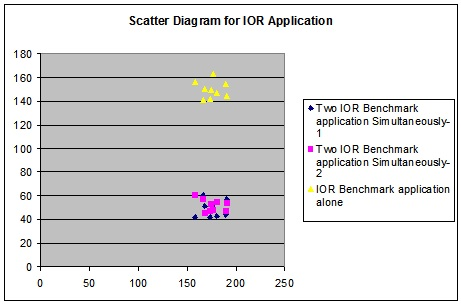
\includegraphics[width=0.5\textwidth]{IOR-Scatter.jpg}
  \caption{Scattered Bandwidth of IOR alone and two IOR running simultaneously, The scattering Shows Two IOR applications running Simultaneously decreased the I/O Bandwidth because of I/O contention}
\end{figure}

\section{Scheduling Policy Based on I/O Bandwidth}
\paragraph{}In the Figure-7 we compared earlier and modified OAR Batch schedulers Job Submission Commands with the Virtual Resource \typebf {bw (Bandwidth)}. It will classify the Job submission with the I/O requirements of each Jobs. In the new scheduling we get the information from the users Number of Nodes and I/O Bandwidth requirement for the Jobs to finish. With that I/O bandwidth information we can avoid the high I/O contention situation by combining Low I/O jobs with Low or High I/O Jobs only to satisfy the full bandwidth of the I/O Bandwidth(bw) resources. In this new approach we eliminated the situation of High I/O and High I/O Jobs combination as well we gave priority to the Job combinations 1) Low and Low I/O Jobs 2) Low and High I/O Jobs. These two priority is mainly reason for the Productivity.


For example in the scenario, sequence of job submissions at the same time is given in the order (Job Id \slash IO Bandwidth), here the nodes and walltime are same for all the Jobs. The lists as follows
(1/80),(2/70), (3/30), (4/20), (5/40), (6/20), (7/40). In the earlier scheduling approach requested number of nodes are available then it will allocate all the Jobs at the same time as mentioned in the Figure-8 irrespective of the I/O requirements of the each applications.


In the new scheduling approach we combined Low I/O Jobs with Low I/O or High I/O with the productivity concern then the jobs will be delayed for assigning Computing nodes, Even though Computing nodes are available. This delay(waiting) for assigning resources due to the reason of "bw" resource exhaustion in the system. Until the bandwidth is available, all the jobs will be in the "Waiting" state to avoid I/O contention. After the "bw" resource was available again it will check in the "Waiting"state Jobs pool to select best suitable Jobs to satisfy the low I/O contention in the system. In this scheduling we are giving high priority to the Low I/O Jobs so high I/O Jobs may not get a chance (Starvation) to run, while high number of Low I/O Job requests in the "Waiting" Job pool. Resolving the problem we can take the time for Job submission is another Priority so the Starvation will not be that much high. In Figure-9 we have followed all the new procedures above and allocated the Jobs in the different Timings so I/O contention decreased considerable amount and the Productivity will be higher than the previous scheduling method.
\newline
\begin{figure}
  \centering    
      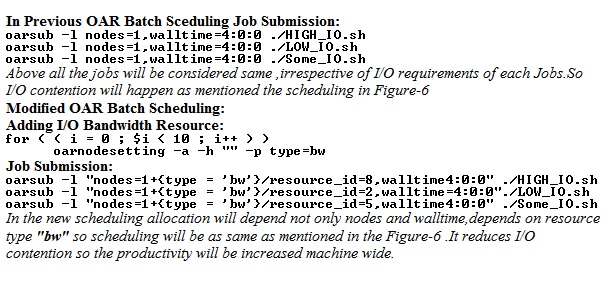
\includegraphics[width=0.5\textwidth]{Commands.jpg}
  \caption{ "oarsub" is the user command in OAR scheduler to submit Jobs. With the above commands we added resources "bw" and compared the previous Scheduling with the New Scheduling Policy. }
\end{figure}
\newline
\begin{figure}
  \centering    
      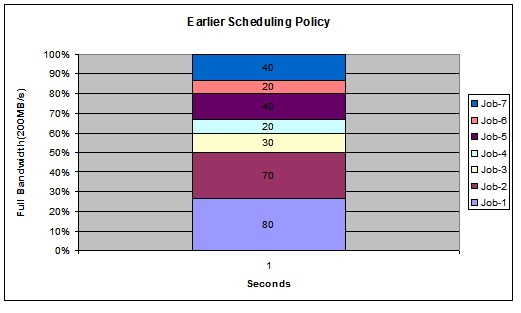
\includegraphics[width=0.5\textwidth]{Theoretical-Earlier-Scheduling.jpg}
  \caption{In the earlier Scheduling Policy. If Computing Nodes are available then it will allocate jobs irrespective of the applications I/O requirement. It causes I/O contention and not good for the machine wide performance. }
\end{figure}
\begin{figure}
  \centering    
      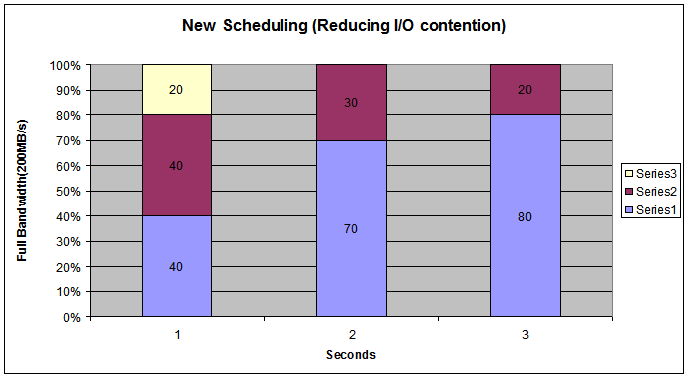
\includegraphics[width=0.5\textwidth]{New-Scheduling-Good.png}
  \caption{In the new scheduling policy we concerned about the jobs I/O operations. From this new approach we avoided high I/O contention scenarios by Scheduler. It reduces I/O contention rate and increased the productivity machine wide.}
\end{figure}
This scheduling approach based on the I/O requirements of each applications. We left the I/O bandwidth requirement to the User, so in the Batch Scheduler simple I/O analysis to segregate the jobs easily. Otherwise we have to keep track of the jobs real I/O requirements History maintained in oar log files to predict the I/O of the applications required for each Jobs. This is the extra work for the Batch Scheduler and costly to predict from the Data. After we got the request we have to choose jobs from the "Waiting" state to fulfill the new scheduling strategy to allocate resources for the jobs in the "Waiting" Job queue to increase the productivity without any starvation for High I/O Jobs in the queue.
\section{Conclusion}
\paragraph{}High I/O contention affects the performance and productivity of the System highly. High I/O contention happens in certain situations when two high I/O jobs request the data from Shared File System (NFS). Avoiding high I/O  contention situations will reduce the I/O contention drastically(from the Section 1 Details), so we can guarantee the performance of the application and productivity of the System. Avoiding high I/O  contention situations by changing the scheduler to support Low I/O Jobs with Low I/O Jobs or High I/O Job to allow multiple processes with low I/O contention. This new scheduling strategy will give good productivity compared to the previous scheduling strategy from the analysis of I/O contention(from the Section 1 Details) with the IOR benchmark and non-application side optimized Jobs. This paper will not free I/O contention completely in the HPC system but it reduces drastically(almost half) to increase the Productivity.   
\section{Future Work}
\paragraph{}We did all the experiments in the context of "Write" based Jobs. Read I/O rate is lower than the Write I/O rate in the most File Systems\cite{IOR_Performance_measurement_in_File_System}. When the "Read" based Job and "Write" based Job run simultaneously then the behavior will change so we have to take into account more constraints(Read and Write based Jobs) to collect data to show what are all the other high I/O contention occurring scenarios and change Scheduling strategy to avoid them by the new scheduling Policy to increase the productivity System wide.

%% The file named.bst is a bibliography style file for BibTeX 0.99c
\bibliographystyle{named}
\bibliography{myreference}
%[1]  http:\/\/en.wikipedia.org/wiki/Distributed\_file\_system \newline\newline
%[2] http:\/\/www.nersc.gov\/users/computational\-systems/nersc-8-system-cori/nersc-8-procurement/trinity-nersc-8-rfp/nersc-8-trinity-benchmarks/ior/ \newline\newline
%[3] A batch scheduler with high level components,Nicolas Capit Georges Da Costa Yiannis Georgiou Guillaume Huard 
%Cyrille Martin Gregory Mounie Pierre Neyron
%Olivier Richard.\newline\newline
%[4] https://www.grid5000.fr/mediawiki/index.php \newline\newline
%[5] [Matthieu Dorie et al, IPDPS 2014]CALCioM: Mitigating I/O Interference in HPC Systems 
%through Cross-Application Coordination \newline\newline
%[6]http://oar.imag.fr/dokuwiki/doku.php?id=wiki:building\_a\newline
%\_demo\_cluster\_using\_docker \newline\newline
%[7] http://www.docker.com/whatisdocker/ \newline\newline

\end{document}

